%%%%%%%%%%%%%%%%%%%%%%%%%
% THIS HEADER needs to remain UNCHANGED
%%%%%%%%%%%%%%%%%%%%%%%%%
\documentclass[a4paper,preprint]{sig-alternate-xt}

\usepackage{times}
\usepackage{helvet}
\usepackage{courier}
\usepackage{microtype}
\usepackage{graphicx}
\usepackage{forest}
\usepackage{tikz-qtree}
\usepackage[numbers]{natbib}
\usepackage{lscape}


%OWN PACKAGES
\usepackage{svg}
\usepackage{xurl}
\usepackage{graphicx}
\usepackage{lipsum}% example text
\usepackage{makecell}

\newtheorem{exmp}{Example}[section]
\usepackage{array}
\newcolumntype{?}{!{\vrule width 1.7pt}}


%%%%%%%%%%%%%%%%%%%%%%%%%
% END HEADER
%%%%%%%%%%%%%%%%%%%%%%%%%


%\frenchspacing

\toappear{}


\usepackage{blindtext}

\begin{document}


\title{A comparison of OSDT, GOSDT and IDS Algorithms}


\numberofauthors{2}
%
\author{
%
\alignauthor Gideon Vogt\\
       \email{gvogt@uos.de}
       
\alignauthor Marcel Hündorf\\
       \email{mhuendorf@uos.de}
}




\maketitle

\begin{abstract}
\begin{quote}
There are numerous interpretable machine learning algorithms available today. We want to test and compare the three implementations Optimal
Sparse Decision Trees (OSDT), Generalized and
Scalable Optimal Sparse Decision Trees (GOSDT) and a python implementation of Interpretable Decision Sets (PyIDS) in regards to accuracy, computing time and understandability. We also want to look at how consistently the algorithms perform well on datasets of different sizes and kinds. To do this we found five different datasets on which we can use the algorithms for binary classification. We preprocessed the datasets in order to create pieces of those datasets of different sizes, with balanced amounts of both classes. For some algorithms we had to create binary versions of these datasets. We then ran experiments with the algorithms for different regularizations for GOSDT and OSDT and different PyIDS algorithms and compared the results.

Results: In regards to accuracy and execution time OSDT has been the best algorithm on these datasets. GOSDT is slightly less accurate and is significantly slower. The PyIDS algorithms performed the worst, with Deterministic Local Search (DLS) being faster but rather inaccurate, and Smooth Local Search (SLS) having good results sometimes but being the slowest algorithm of them all by far. GOSDT and DLS produce the most understandable output of these. 
\end{quote}
\end{abstract}

%------------------------------------------------Introduction-----------------------------------------------
\section{Introduction}
\label{sec:into}
A lot of machine learning models are black boxes. These types do either not explain their predictions at all or do it in a way that humans do not understand. Explainable machine learning tries to explain the black box model by attaching another module to the end.
This can lead to unreliable and misleading explanations.
Severe consequences may follow \cite{BBml}.
To prevent this, models that are inherently explainable are needed.
Interpretable machine learning offers numerous ways of solving this issue.
In this term paper we present and compare three implementations of them in terms of execution time, prediction accuracy, consistency of results on differently sized datasets, interpretability and ease of use.
One of them follows a rule based approach by learning Interpretable Decision Sets (IDS) \cite{IDS}.
\citet{pySchwachsinn} have created a python implementation (PyIDS) which we investigate. Another approach is to generate decision trees.
Here we examine two different methods. The Optimal Sparse Decision Trees (OSDT) Algorithm by \citet{OSDT} and a Generalized and Scalable Optimal Sparse Decision Trees (GOSDT) Algorithm by \citet{GOSDT}.

First, in section \ref{sec:notations} we mention some of the most important notations and describe them.
In section \ref{sec:algorithms} we give a brief overview on how each of the three algorithms works.
Next we give some more details on what datasets the algorithms were trained on in section \ref{sec:data}.
Further in section \ref{sec:prepro} we discuss how these datasets had to be preprocessed. In section \ref{sec:eval} we compare the results obtained by the tests performed. Finally, in section \ref{sec:conclusion} we summarize our findings and provide an outlook to further research.

%--------------------------------------------------Literals-------------------------------------------------


\section{Notations}
\label{sec:notations}
To begin with, in this section the most important notations and terms are explained to build a foundation to work with.
Machine learning (ML) is the study of computer algorithms that can improve automatically through experience and by the use of data. \cite{ML}
Training data can be seen as a table with so called \textsc{attributes} $a_1, \dots, a_i$ as descriptors and \textsc{cases} $c_1, \dots, c_j$ which are the entries.
An attribute $a_k$ describes the $k$-th feature of something whereas a case $c_l$ contains an assigned value for each attribute $a_1, \dots, a_i$. A single entry $e_{kl}$ describes a specific assignment for attribute $a_k$ from case $c_l$, such that $e_{1l}, \dots, e_{jl}$ constructs case $c_l$. The set $V_k$ of all possible assignments for an attribute $a_k$ are called attribute values.
For every training set, there is one special attribute $a_i$ called \textsc{class}.
In the following, an entry for a class always has a binary assignment.
In general, this is not always the case, but it is necessary for the algorithms presented here.
If there would be more than two possible assignment values for a class, the class would be categorizes as a multiclass.

\begin{exmp}
In table \ref{tab:training_data} you can see a table with 5 attributes and 4 cases, which results in $5\cdot4=20$ entries.
Its last attribute ($i$-th attribute) 'is fit' is the class. 'weight' in this example is the attribute $a_1$, the assignments $\{\text{weight}=105, \text{age}=34, \text{job}=\text{DIY store},\text{size}=168,\text{is fit}=true\}$ the case $c_2$ and the entry $\text{job}= none$ is $e_{33}$. Finally the attribute values $V_5$ for the attribute $a_5$ (is fit) is {true/false}.

\begin{table}[h]
\centering
\begin{tabular}{rrcr|c}
\multicolumn{1}{c}{weight} & \multicolumn{1}{c}{age} & job       & \multicolumn{1}{c|}{size} & is fit \\ \hline
60                         & 25                      & student   & 178                       & true   \\
105                        & 34                      & DIY store & 168                       & true   \\
66                         & 25                      & none      & 180                       & false  \\
120                        & 50                      & teacher   & 164                       & false 
\end{tabular}
\caption{Example of a small training dataset about peoples fitness.}
\label{tab:training_data}
\end{table}
\end{exmp}

\section{The Algorithms}
\label{sec:algorithms}
In the following, the basic ideas of the tree algorithms mentioned in section \ref{sec:into} are explained. First, in subsection \ref{subsec:osdt} we start with the Optimal Sparse Decision Trees (OSDT) algorithm which creates optimal decision trees in regards to a so called regularization parameter.
Then in subsection \ref{subsec:gosdt} the more generalized algorithm Generalized and Scalable Optimal Sparse Decision Trees (GOSDT) will be briefly explained and finally, in subsection \ref{subsec:pyschwachsinn} the PyIDS algorithm which has a rule based approach will be outlined.


\subsection{OSDT}
\label{subsec:osdt}
Decision Trees are an easy to understand solution representation to predict cases, since they visually show the decisions path in an intuitive way.
Generating them however is not that simple.
An easy-to-follow example decision tree can be seen in figure \ref{fig:extree}.
\begin{figure}[h]
\begin{forest} for tree={
    edge path={\noexpand\path[\forestoption{edge}] (\forestOve{\forestove{@parent}}{name}.parent anchor) -- +(0,-12pt)-| (\forestove{name}.child anchor)\forestoption{edge label};}
}
[ enemy is dumb 
    [ you are smart 
        [ enemy is cheating 
            [ is bad 
                [ you lose ] 
                [you win ] 
            ] 
            [ you lose ] 
        ]
        [ you win ]
    ]
    [ enemy is cheating 
        [you win]
        [you lose]
    ]
]
\end{forest}
\caption{Example decision tree for a hyptothetical game to predict if you or the enemy will win.
Left path is always false and the right path is always true.}
\label{fig:extree}
\end{figure}

Mathematical programming, greedy, or brute force methods have the disadvantage of either being too computationally hard or have the issue of not being able to revert decisions at the beginning of a decision tree while constructing it top to bottom.

Optimal decision trees for a set of training data are extremely hard to compute and often their computation is not feasible. Not to be confused, the predictions of an optimal decision tree does not have to be optimal, since decision trees are not always able to construct an optimal solution. Often these are also not desired, as they tend to overfit. For these reasons sparse decision trees might be a better solution.

Different to optimal decision trees, a sparse decision tree is optimal, if the value of some optimization function is optimal. For a given decision tree the optimization value results from the misclassification error and a sparsity penalty on the number of leaves. This means, that small trees get preferred.

The OSTD algorithm by \citet{OSDT} does exactly that and always finds the optimal solution for a given so called regularization parameter. It scales how big the penalty is in regards to the size of a tree. The generated tree always makes binary decisions as the attributes of the training set are required to be binary too.

The authors mention, that it is possible to generalize the framework to be able to handle multiclasses too, but considering our datasets (see section \ref{sec:data}) this will not be needed. The OSDT algorithm can be found at \url{https://github.com/xiyanghu/OSDT/commit/4c2049bb70afeffcefe1bb5bf8129e13ec2d8e1a}.

\subsection{GOSDT}
\label{subsec:gosdt}
The previously described OSDT Algorithm is optimized to work with just a single optimization function and only works with binary attributes.
To create a more generalized algorithm, the Generalized and Scalable Optimal Sparse Decision Trees (GOSDT, pronounced 'ghost') Algorithm was created.

It addresses the issue of imbalanced data sets, continuous attributes and multiclasses. Although the additional feature will not be tested in this term paper it is interesting to see if this more general version can compete with the more specific OSDT algorithm or if the generalizations cause problems e.g. in terms of computation time. For the results see section \ref{sec:eval}.

In comparison to other similar implementations GOSDT does not rely on the so called bucketization of continuous attributes. As shown in \cite{GOSDT} this would sacrifice optimality. They solved this issue by using 'similar support'
bounds which "\dots states that if
two features in the dataset are similar, but not identical,
to each other, then bounds obtained using the first feature
for a split in a tree can be leveraged to obtain bounds for
the same tree, were the second feature to replace the first
feature." \cite{GOSDT}

The GOSDT algorithm can be found at \url{https://github.com/Jimmy-Lin/GeneralizedOptimalSparseDecisionTrees/commit/7cc0c061ea7d00fc08c02c1ddc5541eb3255d5e8}


\subsection{PyIDS}
\label{subsec:pyschwachsinn}
PyIDS has a different approach to predict a class.
It aims to learn Interpretable Decision Sets (IDS) which consist of association rules. An association rule is a rule which predicts a class if certain conditions are met. For example: $\text{if } (\text{hot}==\text{true}) \land (\text{color}==\text{brown}) \land  (\text{taste}==\text{good}) \text{ then } \text{class}=\text{coffee}$. Compared to other IDS implementations PyIDS focuses on using submodular function optimization instead of a heuristic.
Fundamentally PyIDS tries to optimize a combination of seven objectives:
\begin{itemize}
    \item decrease the number of rules
    \item decrease the total number of conditions across all rules
    \item decrease the number of overlaps (in terms of instances covered) between rules of the same class
    \item decrease the number of overlaps (in terms of instances covered) between rules of different classes
    \item increase the number of classes which are predicted by at least one rule
    \item decrease the total number of incorrectly covered instances classified by individual rules,
    \item increase the number of data points which are correctly covered by at least one rule.
\end{itemize}

These seven objectives are weighted by lambdas which can be set individually.The PyIDS implementation as well as some examples can be found at \url{https://github.com/jirifilip/pyIDS/commit/c247c08a631c9d47b12bb6972d3540a44f80bd30}

\section{Sets of Data}
\label{sec:data}
To properly train and test the tree algorithms explained in section \ref{sec:algorithms}, different datasets in terms of the number of attributes, their scope of application and type of attribute values have been selected. In the following all five used datasets are described.

\subsection{Chess}
The first dataset is a dataset derived from the game chess and was originally created by \citet{chess}. More specifically it describes cases of a chess end game, where only the white King and Rook and the black King and Pawn are left. This specific variant is usually abbreviated as KRKPA7 (King+Rook versus King+Pawn on a7) and means that the pawn is one tile away from queening and it is the white players turn.

The attributes of this set describe the location of the game pieces on the board. The class finally describes, if the white player has a chance to win or not. The set has in total 3196 cases of which in 1669 (52\%) white can win and in 1527 (48\%) white cannot win.

There are a total of 36 Attributes, some of which are binary and some categorical. The KRKPA7 dataset is provided by \url{https://archive.ics.uci.edu/ml/datasets/Chess+\%28King-Rook+vs.+King-Pawn\%29}.

\subsection{Census Income}
The census dataset displays whether the income of a person exceeds \$50K/yr based on census data. The extraction of the data was done by Barry Becker from the 1994 Census database with the conditions $((\text{AAGE}>16) \land (\text{AGI}>100) \land (\text{AFNLWGT}>1) \land (\text{HRSWK}>0))$. For more information see \url{https://archive.ics.uci.edu/ml/datasets/Adult}.

The attributes describe information about the person such as age, sex, relationship etc. and cover numeric, categorical as well as binary types. The class predicts if the person exceeds an income of \$50K/yr.
It has 32561 cases of which 7841 (24.1\%) predict to exceed \$50K/yr and 24720 (75.9\%) of which they do not. An idiosyncrasy is that there are some missing values.

\subsection{Mushrooms}
The Mushroom datasets describes attributes of North American mushrooms with its class being if they are edible, definitely poisonous or of unknown edibility and not recommended. The latter two values were combined to a value of unsafe to eat.

The data of the mushroom records were drawn from \cite{mushroom}.
This data set includes descriptions of hypothetical samples corresponding to 23 species of gilled mushrooms in the Agaricus and Lepiota Family.
The 23 Attributes are binary and categorical and are assigned with 8124 cases of which 4208 (51.8\%) are edible and 3916 (48.2\%) are not safe to eat. This dataset also includes cases which contain unknown values and is available at \url{https://archive.ics.uci.edu/ml/datasets/Mushroom}.

\subsection{Email Spam}
The Email Spam dataset is a dataset which contains information about received emails. Mark Hopkins, Erik Reeber, George Forman and Jaap Suermondt created this dataset from spam mails drawn from their postmaster and individuals who had filed spam and non-spam mails from filed work and personal e-mails. The all numeric attributes describe the frequency of certain characters, the frequency of a certain word and some additional information. The binary class is if the email was a spam mail or not.

The dataset includes 1813 (39.4\%) cases of spam mails and 2788 (60.6\%) which are not totalling 4601 cases.
In practise false negative predictions are far more worse than false positive ones for this subject.
This dataset was provided by \url{https://archive.ics.uci.edu/ml/datasets/Spambase}.


\subsection{Dota 2}
Dota 2 is a popular computer game with two teams of 5 players. At the start of the game each player chooses a unique hero with different strengths and weaknesses. The 116 Attributes of this dataset describe some general information about the game (like gamemode, casual or competitive etc.) and which hero was picked by which team. All attributes are categorical with most of the heroes not chosen at all since only 10 of the 113 heroes can be picked in a single game (10 players each pick one hero). The data was collected using the Dota2ApiLoader (\url{https://gist.github.com/da-steve101/1a7ae319448db431715bd75391a66e1b}) within 2 hours on the 13th of August, 2016 and is provided at \url{https://archive.ics.uci.edu/ml/datasets/Dota2+Games+Results#}.
The binary class describes which team has won the game.

This big dataset contains 102944 cases of played games of which 48782 (52.3\%) of the games were won by the first team and 43868 (47.7\%) by the second one.

\section{Preprocessing of the Datasets}
\label{sec:prepro}


The data of the sets described in section \ref{sec:data} is provided in a '.csv' format and cannot be used without preprocessing.
In this section we describe what problems we faced and how we solved them.

To begin with, the first step is to reorganize the the data since some algorithms require a very specific format for the data.

In subsection \ref{subsec:attr} the conversion from generic attributes to binary attributes is described and in subsection \ref{subsec:touches} some additional steps and the construction of the test and training sets are explained.

\subsection{Attributes}
\label{subsec:attr}
The OSTD Algorithm requires the possible values for each attribute to be binary.
A format that works well for all algorithms is a '.csv'-style format, where each entry $e_{kl}| 1 < k \leq i, 1 < l \leq j$ is binary such that $e_{kl} \in \{0, 1\}$ (false/true).
Additionally the binary class has to be in the last column and its values also in the form of 0/1 (false/true).
Since not all attribute values of our raw datasets are binary, a preprocessing step is needed to convert them into such.
Different kinds of attribute values however have to be processed differently.
All in all we consider three different types of attributes: Categorical ($a^\mathcal{C}$), numerical ($a^\mathcal{N}$) and binary ($a^\mathcal{B}$) attributes.
Binary attributes are very easy to handle. The only thing to be changed are the attribute values itself, since it is not always guaranteed that they are in the format (0/1).

\subsubsection{Categorical}
Categorical attributes are attributes which values can be put into categories.
This means that there is a set of values $V_{k}$ for a categorical attribute $a^c_k$ containing a finite amount of different values.
For each entry of that attribute applies $e_{kl} \in V_{k}$.
To make all categorical attributes binary we create a new set of binary attributes $B_{k}$ such that for every value $v \in V_{k}$ there is a new attribute $a^{\mathcal{C},bin} \in B_{k}$.
Now every entry $e_{kl}$ can be converted into a series of true or false statements (1/0) in regards to the new set of attributes $B_k$.
Note that for every case there is only one 'true' entry in all categories of $B_k$, since every entry $e_{kl}$ of the initial attribute $a^\mathcal{C}_k$ now has its own Attribute.
If however the number of categories $|V_k|$ are less that 3, the attribute is already binary or unary.
The conversion to values of (0/1) then is trivial, since no new categories have to be created.

\begin{exmp}
Given the categorical attribute $a^\mathcal{C}_1$ 'hair color' with possible values $V_{1} = \{\text{blonde},\text{brown},\text{black},\text{red}\}$.
Then we create binary attributes $B_{1} = \{\text{is\_blonde},\text{is\_brown},\text{is\_black},\text{is\_red}\}$.
For a case where the attribute value of 'hair color' is 'brown', we then get an assignment of the new attributes with 'is\_blonde' = $0$, 'is\_brown' = $1$, is\_black = $0$, 'is\_red' = $0$.
\end{exmp}

\subsubsection{Numeric}
Numeric values have to be treated differently.
There are different possibilities of tackling continuous as well as integral numbers.
For our preprocessing we implemented a similar approach to the GOSDT algorithms internal one.
To create the new set of binary attributes $B_k$ resulting from attribute $a^\mathcal{N}_k$ with continuous as well as integral numbers for its assignments, we first need to create $b$ buckets, where $b$ is the number of binary attributes that will be created from attribute $a^\mathcal{N}_k$.
We then find the upper bound $v^{max}_k$ and the lower bound $v^{min}_k$. For the $n$-th bucket (starting at 1) we create a reference value of $r_{n k} = v^{min}_k + \frac{v^{max}_k-v^{min}_k}{b+1} \cdot n$.
For each entry $e_{kl}$ of attribute $a^\mathcal{N}_k$ we can now create a binary entry $e^{bin}_{n k l}$ for each bucket $n$ corresponding to a new attribute $a^{\mathcal{N}, bin}_{kn}$.
The value of the binary entry $e^{bin}_{n j k}$ corresponding to the $n$-th bucket is true, if $e_{kl}>r_{n k}$ and false otherwise.
By comparing with these reference values we have the advantage to implicitly create $b+1$ intervals with $(-\infty, r_{1 k}], (r_{1 k}, r_{2 k}], \dots, (r_{b k}, \infty)$ by only creating $b$ new attributes.
An exception is made, if there are less different entries for an attribute then there are buckets.
In that case the attribute is handled like a categorical one as described above.

\begin{exmp}
\label{exmp:numeric}
Given the numerical attribute $a^\mathcal{N}_1=$'age' with integral values, 5 cases with entries $15, 23, 45, 50, 56, 75$  for $a^\mathcal{N}_1$ and the number of bins $b=2$.
The lower bound then is $v^{min}_1 = 15$ and the upper bound $v^{max}_1 = 76$.
For the bins reference values we get $r_{11}1 = 15 + \frac{76-15}{3}\cdot1 = 35$ and $r_{21} = 15 + \frac{76-15}{3}\cdot2 = 55$.
Finally we get the binary values by comparing with the reference values shown in table \ref{table:numeric}.
\begin{table}[h]
\centering
\begin{tabular}{r|rr}
\multicolumn{1}{c|}{case value} & \multicolumn{1}{c}{\textgreater{}35} & \multicolumn{1}{c}{\textgreater{}55} \\ \hline
15                              & 0                                    & 0                                    \\
23                              & 0                                    & 0                                    \\
45                              & 1                                    & 0                                    \\
50                              & 1                                    & 0                                    \\
56                              & 1                                    & 1                                    \\
75                              & 1                                    & 1                                   
\end{tabular}
\caption{Resulting attribute values for the new attributes age>35 and age>55 from example \ref{exmp:numeric}.}
\label{table:numeric}
\end{table}
\end{exmp}

\subsection{Final Touches}
\label{subsec:touches}
After the initial preprocessing the data has to be cleaned up.
Some cases of some datasets have undefined or unknown attribute values.
These cases had to be filtered out, otherwise a rule or a decision in a decision tree could be learned where the attribute 'undefined' or 'unknown' matters.

Finally our datasets had to be divided into a dataset to learn from and a dataset to test its accuracy of its predictions.
For our training datasets we have chosen the sizes of 50, 100, 200, 500, and 1000 cases to cover some different sized training datasets.

Since all datasets mentioned in section \ref{sec:data} are fairly large, we  divided the datasets so that each case of the test dataset does not appear in the training data.
Furthermore to create a balanced learning dataset we have chosen to select cases where half of the class assignments are true and the other half are false. All other cases where no entry is missing or undefined are part of the test set.

\section{Results}
\label{sec:eval}

The experiments were run using python 3.8.10 on a Virtual Machine of Ubuntu 20.04.4 64 bit LTS with 4 processor cores and 8 Gigabytes of RAM. The Virtual Machine was run using VMware Workstation 16 Player on a Windows 10 Host machine with 16 GB RAM and an Intel Core i7-8750H CPU @ 2.20GHz with 6 cores and 12 threads. 

\subsection{Configuration of the Algorithms}
\label{subsec:conf}

For the Decision Tree Algorithms we used the standard configurations as they were provided in the github repositories except when it comes to regularization. For GOSDT this means the options cancellation, look\_ahead, similar\_support, feature\_exchange and continuous\_feature\_exchange were used. For OSDT this means we used the "curiosity" metric and used no time limit. For PyIDS we used a rule cutoff of 50 and the simple lambda set of 1 for every value because finding improved lambdas with the algorithm provided in the readme in github took a very long time on our datasets. The regularizations for the Decision Tree algorithms as well as the type of algorithm that PyIDS used were configuration options we made use of and examined. 


%\blinddocument

\begin{figure}[h]
    \centering
    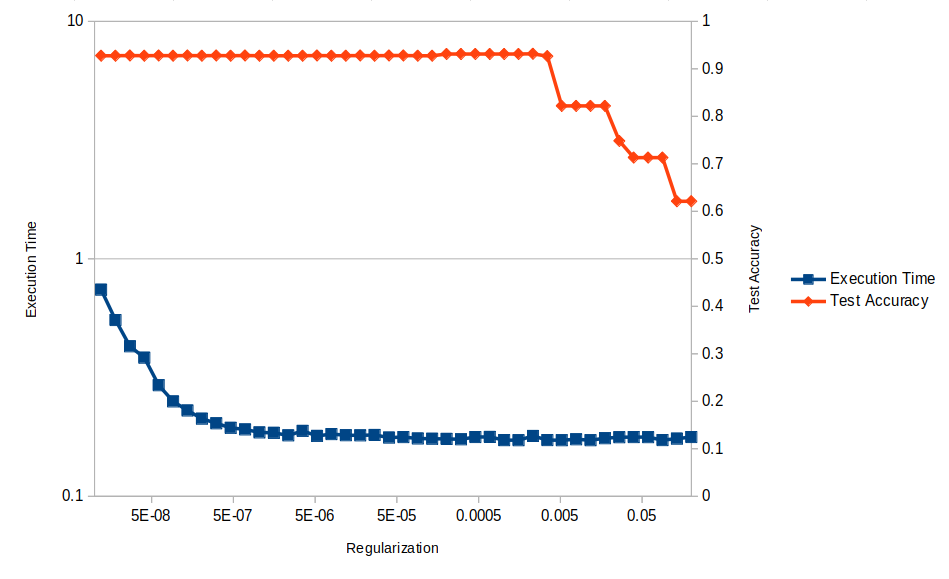
\includegraphics[width=0.5\textwidth]{regtest_osdt.png}
    \caption{The Execution time in seconds and test accuracies of running the OSDT algorithm on the kr-vs-kp dataset trained with 1000 cases with different regularizations.}
    \label{fig:reg1}
\end{figure}

\begin{figure}[h]
    \centering
    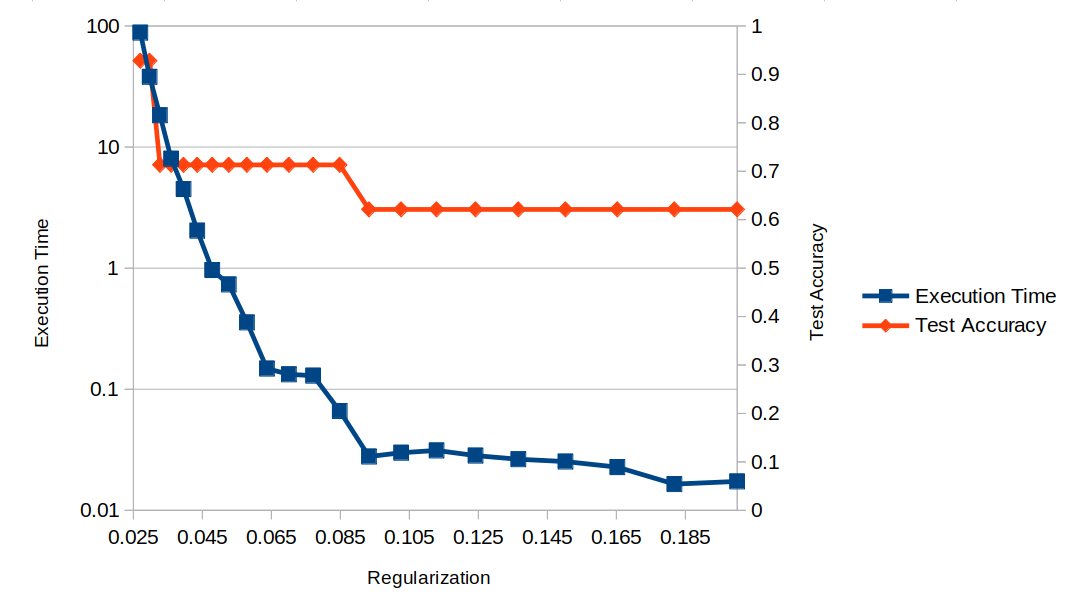
\includegraphics[width=0.5\textwidth]{regtest_gosdt.png}
    \caption{The Execution time in seconds and test accuracies of running the GOSDT algorithm on the kr-vs-kp dataset trained with 1000 cases with different regularizations.}
    \label{fig:reg2}
\end{figure}

As one can see in the images \ref{fig:reg1} and \ref{fig:reg2}, for both the OSDT and GOSDT algorithms a smaller regularization leads to better test accuracies but also higher computation/execution times. The execution times appear to grow exponential with smaller regularizations. 
For the OSDT algorithm there are no further improvements below a regularization value of about 0.001. This is also reflected on other datasets. Because the execution time is still low with this regularization on all datasets, we chose a regularization of $0.0005$ for the OSDT Algorithm for all datasets.

The GOSDT algorithm can take a lot of time with lower regularizations, especially on datasets with many attributes, as in the Dota 2 dataset for example. In the case of the of the kr-vs-kp dataset, a good value for the regularization is for example the standard value of 0.05, because values smaller than this will see much higher runtimes. 
But for other datasets GOSDT a have to set the regularizations differently, as this regularization will cause very long exectuion times for other datasets, as kr-vs-kp has comparably few attributes. We chose the regularization for a dataset with which the algorithm can be trained within a few seconds on the dataset with 1000 entries. For the Dota 2 dataset, the regularization must be chosen so high, that the resulting tree classifies everything as 1. The regularization values for each dataset can be seen in table \ref{table:gosdt_regs}.

\begin{table}[]
\begin{tabular}{l|l}
Dataset          & Regularization \\ \hline
Adult            & 0.07           \\
Agaricus Lepiota & 0.005          \\
Dota 2 Train     & 0.18           \\
kr-vs-kp         & 0.05           \\
Spambase         & 0.055         
\end{tabular}
\label{table:gosdt_regs}
\caption{The Values for regularization that were used for GOSDT on different Datasets.}
\end{table}

For the Agaricus Lepiota dataset GOSDT can use the same regularization as OSDT. This is why the next tests were done on this dataset, for better comparability. 

There are two algorithms that PyIDS can use as mentioned in \cite{pySchwachsinn}. These are Smooth Local Search (SLS) and Deterministic Local Search (DLS). In some experiments we did on the datasets with 1000 cases SLS tended to be the better algorithm generally, however, it works with random elements and can also yield comparably bad results sometimes. It also takes longer than DLS. DLS is more stable in it's results. We used PyIDS on the binary Datasets and in all cases it resulted in a model that always classified every case as the same of the two options and therefore was a trivial and uninteresting result. Therefore all test results shown for the PyIDS algorithms will be results on the nonbinary datasets, which contain the same cases but technically contain more accurate information, as the binary datasets are binned as described in section \ref{sec:prepro}.

\subsection{Test results}
\label{subsec:testresults}


\begin{figure}[h]
    \centering
    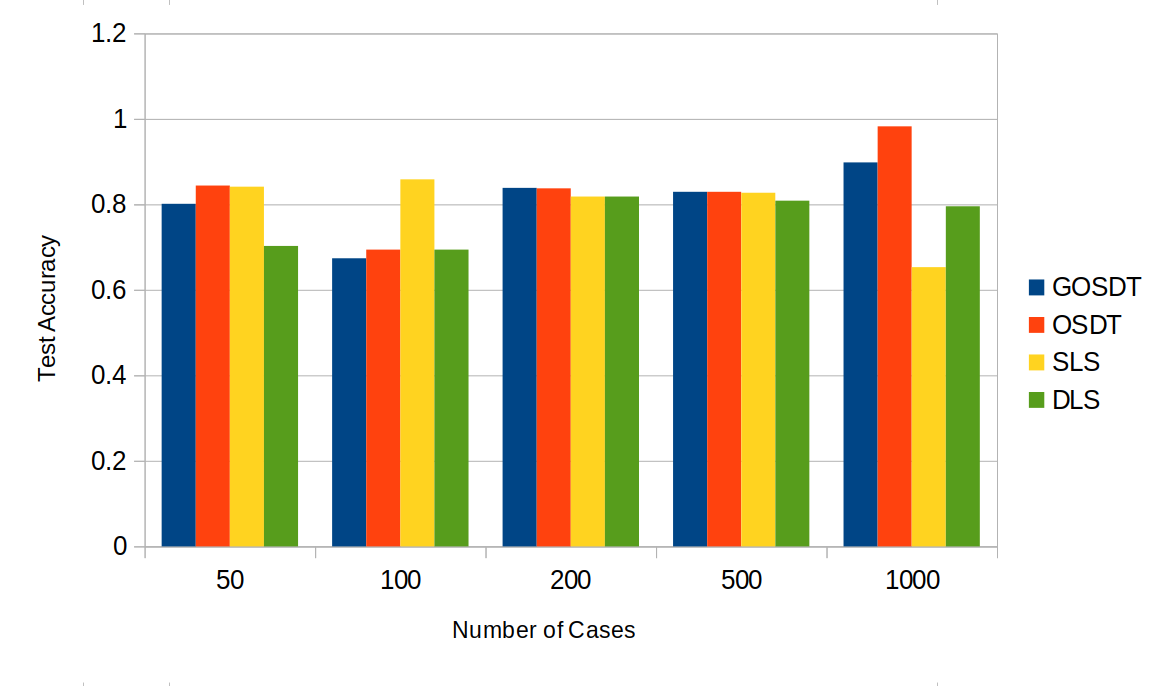
\includegraphics[width=0.5\textwidth]{SizeTests_Acc.png}
    \caption{The test accuracies of the GOSDT, OSDT and PyIDS SLS and DLS algorithms depending on the amount of cases they were trained with on the Agaricus Lepiota dataset.}
    \label{fig:size1}
\end{figure}

\begin{figure}[h]
    \centering
    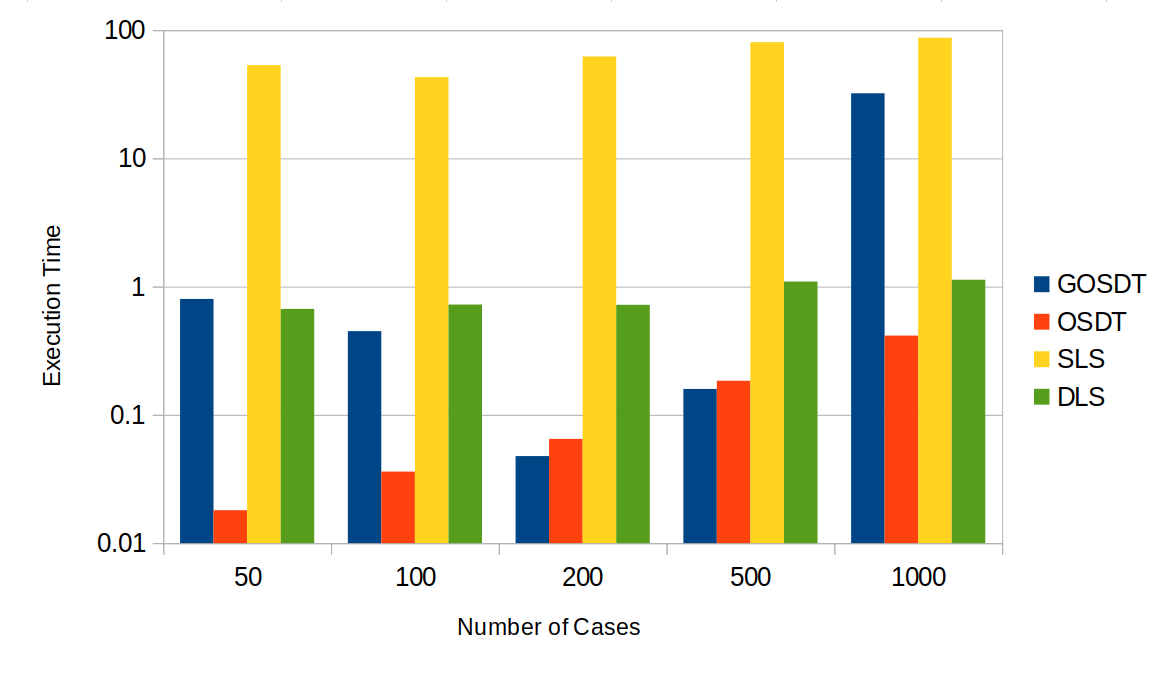
\includegraphics[width=0.5\textwidth]{sizetests_time2.png}
    \caption{The execution times of the GOSDT, OSDT and PyIDS SLS and DLS algorithms depending on the amount of cases they were trained with on the Agaricus Lepiota dataset on a logarithmic scale.}
    \label{fig:size2}
\end{figure}

Figures \ref{fig:size1} and \ref{fig:size2} show the test accuracies and execution times of GOSDT, OSDT and PyIDS with SLS and DLS on 5 different datasets based on the Agaricus Lepiota dataset. The x-axis shows how many cases the dataset used for training the algorithm had. Figure \ref{fig:size1} shows how the test accuracies on this dataset generally are quite comparable among all four algorithms. GOSDT, OSDT and DLS seem to show at least a small positive corrrelation between the number of cases and test accuracies, even though this is not always given, as the accuracies for all three of these algorithms are lower on the 100 dataset than on the 50 dataset. For SLS, it seems as if there is a negative correlation, however, this can also be due to the random nature of this algorithm. On the 1000 dataset OSDT is however the clear winner achieving a text accuracy very close to 100\%. On some datasets SLS can be much better than the other algorithms with some luck as shown on the 100 Dataset, so if one used SLS a consecutive number of times on a dataset, one might achieve very good results with that too.

Figure \ref{fig:size2} shows the clear differences between the algorithms when it comes to execution time. In light of the logarithmic scale, it is clear that SLS generally takes much longer than all the other algorithms and this is only slightly affected by the size of the dataset. DLS is a lot faster and very consistent over the differently sized dataset and its runtime also only slightly increased with the growth of the datasets. GOSDT shows no clear correlation between datasets and execution time, other properties of the datasets seem to affect the execution time of GOSDT more strongly. The execution time of OSDT seems to grow clearly and with the number of the cases. Yet, it is still the fastest on most datasets, including the biggest one. On this dataset it is also the clearest how GOSDT can be much slower than OSDT.

\begin{table}[]
\begin{tabular}{l?lll}
Algorithm        & GOSDT          &           &          \\
Dataset          & Execution Time & Train Acc & Test Acc \\ \hline
Adult            & 36.09          & 0.78      & 0.70     \\
Agaricus Lepiota & 5.16           & 1.00      & 0.81     \\
Dota 2           & 2.45           & 0.50      & 0.47     \\
Kr-vs-kp         & 0.08           & 0.91      & 0.70     \\
Spambase         & 4.24           & 0.72      & 0.75     \\ \hline
Average          & 9.60           & 0.78      & 0.69     \\ \Xhline{3\arrayrulewidth}
Algorithm        & OSDT           &           &          \\
Dataset          & Execution Time & Train Acc & Test Acc \\ \hline
Adult            & 0.15           & 0.91      & 0.72     \\
Agaricus Lepiota & 0.13           & 1.00      & 0.85     \\
Dota 2           & 0.42           & 0.82      & 0.51     \\
Kr-vs-kp         & 0.06           & 0.98      & 0.81     \\
Spambase         & 0.18           & 0.83      & 0.76     \\ \hline
Average          & 0.19           & 0.91      & 0.73     \\ \Xhline{3\arrayrulewidth}
Algorithm        & DLS            &           &          \\
Dataset          & Execution Time & Train Acc & Test Acc \\ \hline
Adult            & 2.12           & 0.59      & 0.40     \\
Agaricus Lepiota & 0.82           & 0.98      & 0.76     \\
Dota 2           & 9.04           & 0.50      & 0.47     \\
Kr-vs-kp         & 0.74           & 0.86      & 0.70     \\
Spambase         & 5.55           & 0.50      & 0.62     \\ \hline
Average          & 3.65           & 0.68      & 0.59     \\ \Xhline{3\arrayrulewidth}
Algorithm        & SLS            &           &          \\
Dataset          & Execution Time & Train Acc & Test Acc \\ \hline
Adult            & 7.82           & 0.64      & 0.52     \\
Agaricus Lepiota & 59.94          & 0.97      & 0.83     \\
Dota 2           & 41.49          & 0.50      & 0.47     \\
Kr-vs-kp         & 26.81          & 0.89      & 0.68     \\
Spambase         & 12.38          & 0.50      & 0.62     \\ \hline
Average          & 29.69          & 0.70      & 0.62    
\end{tabular}
\label{table:allvals}
\caption{A table containing all average execution times, training accuracies and test accuracies of the different algorithms on different datasets.}
\end{table}

In table \ref{table:allvals} one can see the average values for the execution time, training accuracy and test accuracy of GOSDT, OSDT, DLS and SLS on the five different datasets, including the five datasets with different numbers of cases each, and the average over all five datasets in total. It should be noted here again, the the PyIDS algorithms SLS and DLS use the nonbinary versions of the datasets and OSDT and GOSDT use the binary versions. When ranking these algorithms by their average test accuracy, OSDT is first, GOSDT is second best, SLS is third and DLS is last. One can see that OSDT is better than SLS, DLS and GOSDT on every dataset in this regard. SLS is better than GOSDT on the Agaricus Lepiota dataset, but besides that they are equally good or SLS is worse. This shows that in our tests, the Decision Tree algorithms have performed generally better than the PyIDS algorithms and of the two Decision Tree algorithms OSDT is the clear winner when it comes to test accuracy. The train accuracies generally reflect this picture as well.

When it comes to execution time, OSDT is once again the clear winner, being numerous times faster than any other algorithm on average. DLS takes the second place, still generally not overly slow but already much slower than OSDT. GOSDT takes the third place, whereas it is important here, that choosing other regularizations would have led to other results in this regard, as it affects the execution time of GOSDT very directly. So by sacrificing Test accuracy, one could accomplish faster execution times and vice versa. However, most of these regularization values were already chosen so high that putting it any higher would result in execution times of multiple minutes or hours very quickly. 
SLS takes the last place, it takes multiple seconds on all datasets and up to one minute on the Agaricus Lepiota dataset.

This shows the OSDT is both in regards to execution time and accuracy the best algorithm of them all on these datasets. GOSDT could probably be faster than DLS and still be better than it with smaller regularization values, therefore it performs better than DLS in general. Of DLS and SLS, DLS is the faster one and SLS the more accurate one. This difference would be exaggerated by using SLS in a Monte Carlo Scheme, meaning the algorithm will be executed multiple times and the best result will be kept, the runtime would become even bigger but overly bad results due to chance would be significantly reduced.  
By improving the preprocessing of the Data, the performance  of the Decision Tree algorithms possibly could be improved further. The PyIDS algorithms unfortunately did not work on binarized datasets at all, besides classifying all cases in the same way. 


Bigger datasets like Dota 2 can quickly become too large for the GOSDT algorithm. The number of attributes is a crucial factor when it comes to this. Even the datasets containing only 50 cases can not be solved quickly by GOSDT with a normal regularization like 0.06. Therefore this dataset was solved with a very high regularization of 0.18, causing the resulting model to be trivial. The PyIDS Algorithms also weren't capable of providing a nontrivial solution for these datasets. OSDT was the only algorithm that managed to construct a nontrivial model for this dataset, but even with that, the test accuracy was barely above 50\%. Adult is also a dataset that is big and not easy to solve as demonstrated by the bad accuracies of the PyIDS algorithms as well as the high execution time of GOSDT despite the slightly higher regularization for it. This shows that big datasets are a challenge for all of these algorithms at some point, while OSDT is the most robust against a large dataset size. On the smaller and less complex datasets "Agaricus Lepiota" and "Kr-vs-kp" all algorithms perform somewhat well, with the Decision Tree algorithms reaching a training accuracy of 1.0. However it is surprising to see that the SLS algorithms execution time on "Agaricus Lepiota" exceeds that of "Dota 2" and that of "Kr-vs-kp" exceeds that of "Adult".

\subsection{Understandability}
\label{subsec:understandability}

GOSDT gives the best and most understandable output. Both the tree representation as well as the rule representation of the model are easily understandable. The trees also are usually not very complex and therefore easy to understand. 
OSDT also uses trees, these however tend to be more complex and the way OSDT displays them makes it not very easy to understand what the tree actually looks like. Therefore OSDT is initially not easy to understand and even once one does the trees can still be somewhat complex. 
SLS apparently always uses as many rules as it can, so if one chooses to use 50 rules, it's very hard to understand. Not only are the rules not connected as they are in the decision tree, they are also very numerous. All by themselves they tend to be simple and understandable rules though, but the entire set of rules can be hard to understand and overwhelming.
DLS seems to only use one rule most of the time, which is on one hand very understandable, but on the other hand an overly simplistic model, as it will be hard to achieve good accuracies on some datasets with only one single rule. 

\subsection{Ease of Use}
\label{subsec:eou}

This section will describe how easy and intuitive the use of the different Algorithms has been. 

OSDT has been easy to install and use. The installation consisted of downloading and including two python files, and then calling a function. It's usage was clearly presented in example files in the git repository of OSDT. OSDT might work on different operating systems.

GOSDT has not been easy to install at all. The repository has a Setup.py file, making it possible to install it with pip from the Repository. This enables the user to use the C++ extension and build a model/tree. However, this extension provides no methods to evaluate the constructed tree. For this, the user needs to copy or import certain python files from the repository withing the model folder. This python wrapper provides the score function in order to evaluate accuracy and also provides a function for building a model. There are also installation scripts within the git repository. These however did not work for either of us due to numerous errors, caused confusion and also only work on Linux systems. As the only way of installation that is described in the readme uses the installation scripts, the installation was a lengthy process. And because there are basically two versions of the program, one being the C++ extension and the other one being the python wrapper, the right way to use this program was not clear immediately aswell. This essentially provides the user with two fit methods for building a model. We even came across the case that the C++ extension was able to fit some nonbinary datasets for which the python wrapper ran into an error. So there might be further differences or even bugs in the two implementations. This makes the usage a bit confusing and inefficient, however the code-example given in the repository for the python wrapper is a helpful example. If the other problems are overcome the program can be used well, if there are no errors when applying it to datasets.

Technically GOSDT is capable of utilizing multiple cores, however it often runs into endless loops when you want to to use it on data while using multiple cores/threads and therefore we chose to just use one single core for our experiments. 

PyIDS was easy to install, as it could be directly installed using pip. The usage was also easy in itself, given the example code in the readme on the git repository. PyIDS not working on the binary datasets at all caused some extra attention being spent on whether it is being used right or whether the change of some parameters could yield better results. 

\section{Conclusions}
\label{sec:conclusion}
It appears that OSDT is by far the most useful algorithm for these datasets with these sizes. GOSDT can sometimes perform better on some of these datasets however. The authors themselves stated in \cite{GOSDT} that the main use of the GOSDT algorithm opposed to OSDT is to deal with imbalanced data and to optimize over continuous variables. These features were not taken advantage of in these tests, and still there were a few instances where GOSDT performed better than OSDT. However in general, if one is not taking advantage of these properties, GOSDT is a considerably slower and less accurate algorithm on most datasets. GOSDT being less accurate is not only due to the higher regularization values that one needs to use to keep the execution time down, but even on the dataset Agaricus Lepiota, where both algorithms could use the same regularization, OSDT performs better. One needs to keep in mind that this is done using binarized and artificially balanced datasets. If one was to use the nonbinary datasets for GOSDT, one might get other results. 
The PyIDS Algorithms generally performed worse than the Decision Tree Algorithms, however they can yield good results under certain circumstances, as SLS has done one the Agaricus Lepiota dataset. DLS is not a bad algorithm in total, but in these tests it has not shown any particular quality that would distinguish it from the other algorithms in a positive way. It's only advantages are that it is more stable in it's classification accuracy, and overly bad results are more rare than with SLS and it is also faster than SLS. 

For the future, it would be interesting to examine the performance of GOSDT on non-binary datasets. It would also be interesting to examine why PyIDS yieled no non-trivial results on all of our binarized datasets and if it can be used on some binary datasets effectively. The performance of the SLS Algorithm inside a Monte Carlo Scheme could also be worth examining, as it can achieve results that are better than those of the Decision Trees, so possibly, it could reach equal or even better accuracies. 

%\bibliographystyle{acm}
\bibliographystyle{plainnat}
\bibliography{bibliography}

\clearpage

\section{Who did What?}
\begin{itemize}
    \item Gideon Vogt
    \begin{itemize}
        \item abstract
        \item section \ref{sec:eval}: Results
        \item section \ref{sec:conclusion}: Conclusion
        \item programming
            \begin{itemize}
                \item Experiment.py ('term paper/python project/src/experiment.py')
                \item Running experiments and Visualizing Results (Data in 'term paper/python project/libreoffice')
            \end{itemize}
    \end{itemize}
    \item Marcel Hündorf
    \begin{itemize}
        \item section \ref{sec:into}: Introduction
        \item section \ref{sec:notations}: Notations
        \item section \ref{sec:algorithms}: Algorithms
        \item section \ref{sec:data}: Sets of Data
        \item section \ref{sec:prepro}: Preprocessing of the Dataset
        \item programming
        \begin{itemize}
            \item preprocessing (files 'term paper/python project/src/read\_write/util/unify\_datasets.py', 'term paper/python project/src/read\_write/new\_preprocessor.py')
            \item generation of training and test sets (file 'term paper/python project/src/read\_write/dataset\_generator.py')
            \item reader functions (file 'term paper/python project/src/read\_write/reader.py'
        \end{itemize}
    \end{itemize}
    \item together (Vogt/Hündorf)
    \begin{itemize}
        \item picking datasets 50/50
        \item Examining initial Installation and Usage of Algorithms 85/15
    \end{itemize}
\end{itemize}


\end{document}